%% rnaastex.cls is the classfile used for Research Notes. It is derived
%% from aastex61.cls with a few tweaks to allow for the unique format required.
\documentclass{rnaastex}

\usepackage{graphicx}
\usepackage[suffix=]{epstopdf}
\usepackage{natbib}
\usepackage{amsmath}
\usepackage{xspace}

% make the word Kepler italicized, deal w/ floating space afterwards
\newcommand{\Kepler}{\textsl{Kepler}\xspace}


\begin{document}


\title{Infrared Flares on M Dwarfs: a Hinderance to\\ Future Transiting Exoplanet Studies}

%% Note that the corresponding author command and emails has to come
%% before everything else. Also place all the emails in the \email
%% command instead of using multiple \email calls.
\correspondingauthor{James. R. A. Davenport}
\email{jrad@uw.edu}

\author{James. R. A. Davenport}
\altaffiliation{NSF Astronomy and Astrophysics Postdoctoral Fellow}
\altaffiliation{DIRAC Fellow}
\affiliation{Department of Physics \& Astronomy, Western Washington University, 516 High St., Bellingham, WA 98225, USA}
\affiliation{Department of Astronomy, University of Washington, Seattle, WA 98195, USA}


%% Note that RNAAS manuscripts DO NOT have abstracts.
%% See the online documentation for the full list of available subject
%% keywords and the rules for their use.
\keywords{editorials, notices --- 
miscellaneous --- catalogs --- surveys}



%% Start the main body of the article. If no sections in the 
%% research note leave the \section call blank to make the title.
\section{} 

many current and future missions are pushing to infrared (IR) wavelengths to study exoplanets. the motivation for this includes both studies of features in planetary atmospheres where the flux contrast between the planet and star is more favorable \citep{deming2009}, and the decreased impact of stellar activity. Indeed, recent analysis of stellar activity, specifically starspots and faculae, found to not substantially impact the transit signatures from FGKM stars with JWST \citep{zellem2017}. However, this is not true in the case of flares. flares have already been a roadblock for detecting transits for stars in the optical \citep[e.g. Proxima b][]{davenport2016a, kipping2017}.

Dedicated observations by \citet{tofflemire2012} put upper limits on flare flux in the IR for mid-M dwarfs from for moderate amplitude events.
\citet{davenport2012} created peak-flux conversions between $ugrizJHK$-bands for M0--M6, which imply very small amplitudes for IR compared to the dramatic events in the optical.

infrared flares have been observed now, most notably in the transit observations of TRAPPIST-1. This system is an M8, hosting 7 transiting exoplanets discovered by ground- and space-based monitoring \citep{gillon2016,gillon2017}
follow-up data from \Kepler/K2 able to find period of outer planet \citep{luger2017} and recovered many flares for this active low-mass star \citep{vida2017}. 
BOTH the IR and the Optical data contain flares that partially overlap transits: TRAPPIST-1b in the IR from \citet{gillon2017} and TRAPPIST-1h in the optical from \citet{luger2017}.
Figure \ref{fig:1} shows examples, plus the typical figure of merit for flare occurrence, showing powerlaw behavior in both the optical and IR, and with comparable occurrence frequency. 


Since flares are common for low-mass stars, and can occur even for ``inactive'' stars \citep[e.g.][]{hawley2014}, we suggest that future surveys include optical monitoring during transits to help calibrate out the effects of flares. Because flares are significantly higher amplitude in the optical, this monitoring need not be to the same photometric precision, and can likely be done from the ground.




%% An example figure call using \includegraphics
\begin{figure*}[h!]
\begin{center}
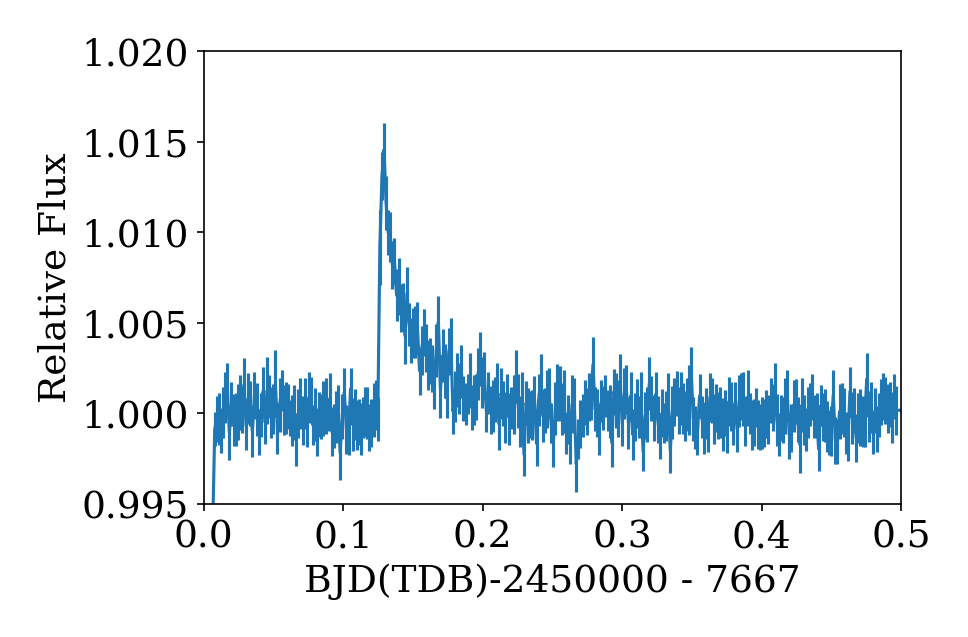
\includegraphics[height=2in]{trappist1_flare3}
\includegraphics[height=2in]{flare_29}\\
\includegraphics[width=4in]{ffd_ED}
\caption{Top: Flares from Spitzer (left) and K2 (right) on TRAPPIST-1. 
Bottom: Cumulative flare frequency distributions for both Spitzer and K2 flare events in units of Equivalent Duration, which can be converted to event energies by 
\label{fig:1}}
\end{center}
\end{figure*}



\acknowledgments

JRAD is supported by an NSF Astronomy and Astrophysics Postdoctoral Fellowship under award AST-1501418. 


%%%%%%%%%%%%%%%%%
\bibliography{/Users/davenpj3/Dropbox/references.bib}

\end{document}
